\subsection {Base de données}

\begin{figure}[h!]
    \centering
    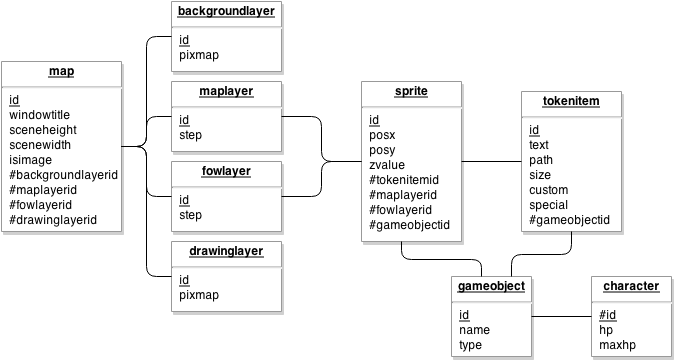
\includegraphics[width=\textwidth]{img/bdd_MLD.png}
    \caption{Modèle Logique des Données}
    \label{fig:bddmld}
\end{figure}

Une base de données PostgreSQL doit être installée avec l'application pour que celle-ci fonctionne correctement. Un script présent dans \textbf{resource/Queries/init.sh} permet d'exécuter les requêtes présentes dans les fichiers initTables.sql et initRows.sql qui, respectivement, permettent de créer les tables et de peupler la base de données. Les tables créées sont modélisées plus haut sur la figure \ref{fig:bddmld}.\\

\begin{figure}[h!]
    \centering
    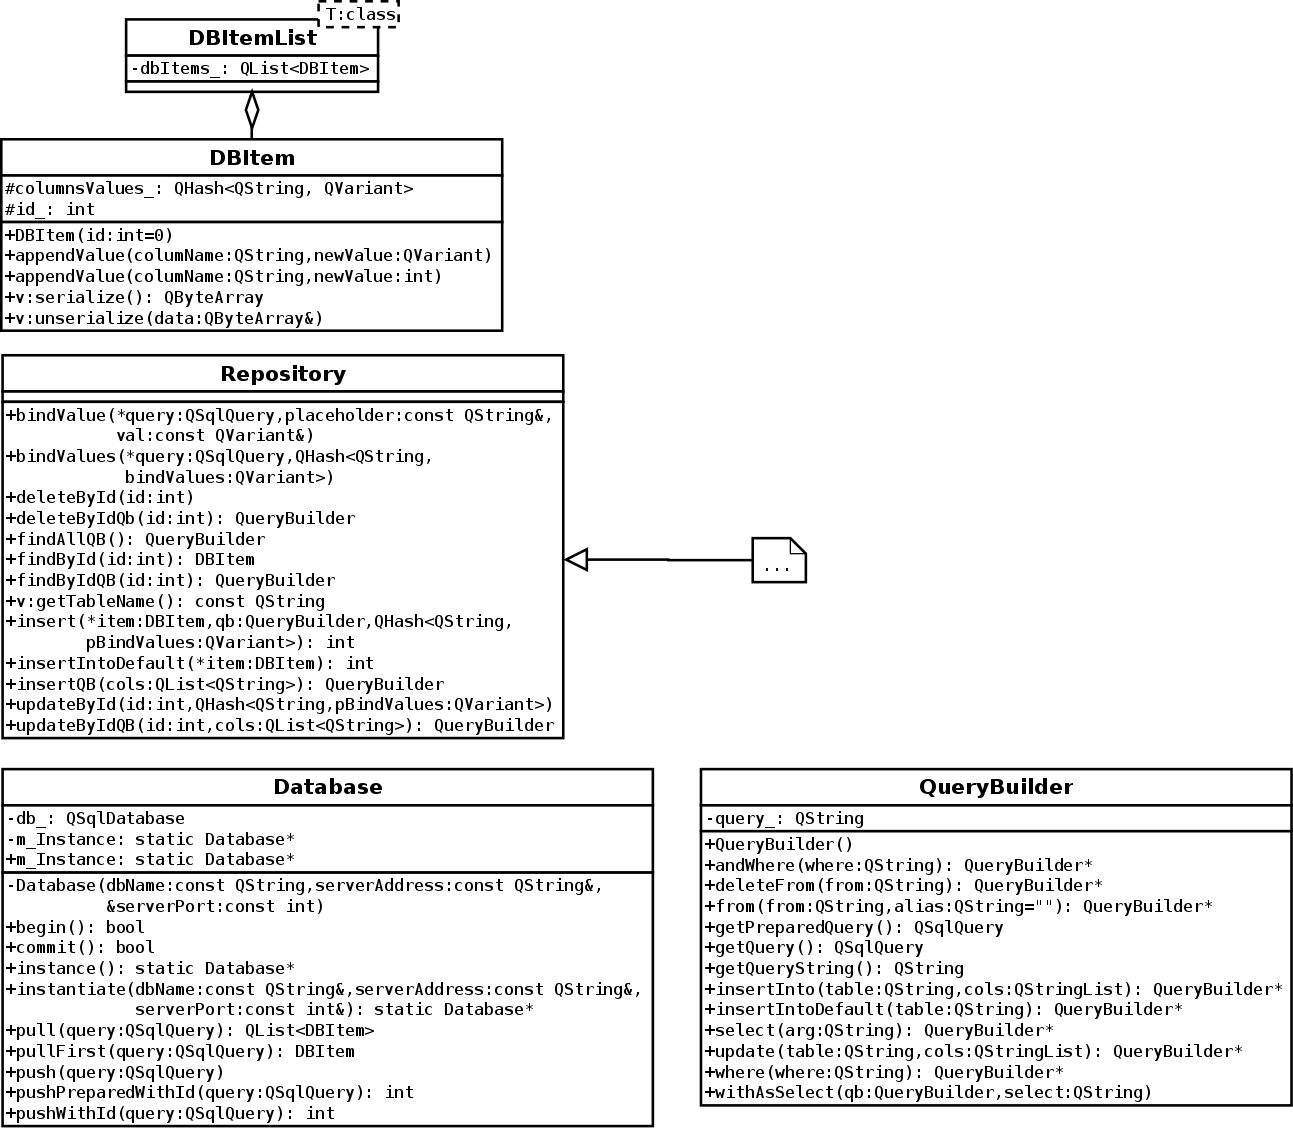
\includegraphics[width=\textwidth]{img/bdd_uml.png}
    \caption{Diagramme UML de la partie BDD (Les classes héritant de Repository ne sont pas représentées pour éviter de surcharger le schéma.)}
    \label{fig:bdduml}
\end{figure}

La base de donnéees est représentée dans l'application par la classe Database qui a été conçue selon le patron de conception Singleton : Database ne peut être instanciée qu'une seule fois. De plus cette instance est accessible à l'ensemble de l'application ce qui évite de devoir passer cette dépendance à un nombre important de classes. Cette classe permet d'effectuer plusieurs opérations sur la bdd PostgreSQL telles que la récupération d'une seule ligne (\emph{pullFirst}), de plusieurs lignes (\emph{pull}), l'exécution d'une requête ne renvoyant pas de résultat (\emph{push}), et l'exécution d'une requête effectuant une opération d'insertion et renvoyant l'id de la ligne insérée (\emph{pushWithId}).\\

Une classe QueryBuilder a été créée afin de faciliter la création de requêtes. Elle permet de chaîner plusieurs chaînes de caractères afin de former une requête complète. Ainsi, des parties de requêtes peuvent facilement être réutilisées et ainsi éviter de la duplication de code.

\begin{lstlisting}[caption=Exemple d'utilisation de QueryBuilder]
QueryBuilder Repository::findByIdQB(int id) {
    QueryBuilder qb;

    qb.select("*")
    ->from(getTableName())
    ->where("id = " + QString::number(id));

    return qb;
}
\end{lstlisting}

\begin{lstlisting}[language=SQL,caption=Equivalent en SQL de la requête créée avec le QueryBuilder]
SELECT * FROM nomDeLaTable 
WHERE id = idDeLaLigne;
\end{lstlisting}

Ces requêtes sont créées dans des classes héritant de Repository. Un Repository et les classes qui en héritent sont des conteneurs de requêtes. La classe de base Repository possède quelques méthodes génériques qui permettent par exemple de récupérer un élément de la base de données par son id (\emph{findById}), ou encore d'insérer une ligne dans la BDD (\emph{insert}). Les classes héritant de Repository peuvent ensuite redéfinir et/ou réutiliser ces méthodes pour les adapter à leurs besoins. Chaque classe pouvant manipuler des objets associés dans la BDD possède un Repository, par exemple la classe Sprite est associée à la table sprite de la BDD et peut manipuler cette table à l'aide des requêtes de SpriteRepository. Enfin, tous les repositories sont accessibles de manière statique depuis la classe RepositoryManager, ainsi toute l'application a accès à ceux-ci.\\

Les classes possédant une table équivalente en BDD (par exemple la classe TokenItem est liée à la table tokenitem) héritent de DBItem. Un DBItem possède une hashmap associant un nom de colonne à sa valeur. Cette hashmap est remplie et sérialisée avant une insertion en base de données, et déserialisée lors de la récupération de lignes de la BDD.